% Created by tikzDevice version 0.10.1 on 2019-05-06 17:18:24
% !TEX encoding = UTF-8 Unicode
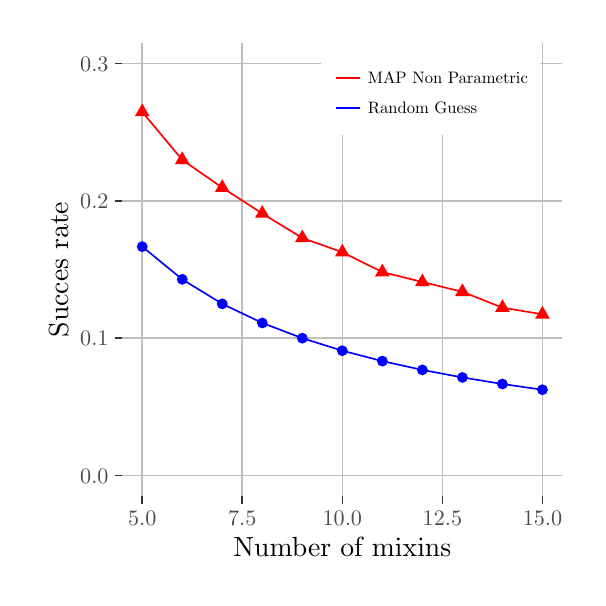
\begin{tikzpicture}[x=1pt,y=1pt]
\definecolor{fillColor}{RGB}{255,255,255}
\path[use as bounding box,fill=fillColor,fill opacity=0.00] (0,0) rectangle (198.74,198.74);
\begin{scope}
\path[clip] (  0.00,  0.00) rectangle (198.74,198.74);
\definecolor{drawColor}{RGB}{255,255,255}
\definecolor{fillColor}{RGB}{255,255,255}

\path[draw=drawColor,line width= 0.6pt,line join=round,line cap=round,fill=fillColor] (  0.00,  0.00) rectangle (198.74,198.74);
\end{scope}
\begin{scope}
\path[clip] ( 34.16, 29.45) rectangle (193.24,193.24);
\definecolor{drawColor}{RGB}{255,255,255}

\path[draw=drawColor,line width= 0.3pt,line join=round] ( 34.16, 61.71) --
	(193.24, 61.71);

\path[draw=drawColor,line width= 0.3pt,line join=round] ( 34.16,111.34) --
	(193.24,111.34);

\path[draw=drawColor,line width= 0.3pt,line join=round] ( 34.16,160.98) --
	(193.24,160.98);

\path[draw=drawColor,line width= 0.3pt,line join=round] ( 59.47, 29.45) --
	( 59.47,193.24);

\path[draw=drawColor,line width= 0.3pt,line join=round] ( 95.62, 29.45) --
	( 95.62,193.24);

\path[draw=drawColor,line width= 0.3pt,line join=round] (131.78, 29.45) --
	(131.78,193.24);

\path[draw=drawColor,line width= 0.3pt,line join=round] (167.93, 29.45) --
	(167.93,193.24);
\definecolor{drawColor}{RGB}{190,190,190}

\path[draw=drawColor,line width= 0.6pt,line join=round] ( 34.16, 36.89) --
	(193.24, 36.89);

\path[draw=drawColor,line width= 0.6pt,line join=round] ( 34.16, 86.53) --
	(193.24, 86.53);

\path[draw=drawColor,line width= 0.6pt,line join=round] ( 34.16,136.16) --
	(193.24,136.16);

\path[draw=drawColor,line width= 0.6pt,line join=round] ( 34.16,185.80) --
	(193.24,185.80);

\path[draw=drawColor,line width= 0.6pt,line join=round] ( 41.39, 29.45) --
	( 41.39,193.24);

\path[draw=drawColor,line width= 0.6pt,line join=round] ( 77.54, 29.45) --
	( 77.54,193.24);

\path[draw=drawColor,line width= 0.6pt,line join=round] (113.70, 29.45) --
	(113.70,193.24);

\path[draw=drawColor,line width= 0.6pt,line join=round] (149.86, 29.45) --
	(149.86,193.24);

\path[draw=drawColor,line width= 0.6pt,line join=round] (186.01, 29.45) --
	(186.01,193.24);
\definecolor{fillColor}{RGB}{0,0,255}

\path[fill=fillColor] ( 41.39,119.62) circle (  1.96);

\path[fill=fillColor] ( 55.85,107.80) circle (  1.96);

\path[fill=fillColor] ( 70.31, 98.94) circle (  1.96);

\path[fill=fillColor] ( 84.78, 92.04) circle (  1.96);

\path[fill=fillColor] ( 99.24, 86.53) circle (  1.96);

\path[fill=fillColor] (113.70, 82.01) circle (  1.96);

\path[fill=fillColor] (128.16, 78.25) circle (  1.96);

\path[fill=fillColor] (142.62, 75.07) circle (  1.96);

\path[fill=fillColor] (157.09, 72.35) circle (  1.96);

\path[fill=fillColor] (171.55, 69.98) circle (  1.96);

\path[fill=fillColor] (186.01, 67.91) circle (  1.96);
\definecolor{fillColor}{RGB}{255,0,0}

\path[fill=fillColor] ( 41.39,171.34) --
	( 44.03,166.77) --
	( 38.75,166.77) --
	cycle;

\path[fill=fillColor] ( 55.85,154.05) --
	( 58.49,149.47) --
	( 53.21,149.47) --
	cycle;

\path[fill=fillColor] ( 70.31,143.98) --
	( 72.96,139.40) --
	( 67.67,139.40) --
	cycle;

\path[fill=fillColor] ( 84.78,134.64) --
	( 87.42,130.07) --
	( 82.13,130.07) --
	cycle;

\path[fill=fillColor] ( 99.24,125.79) --
	(101.88,121.22) --
	( 96.59,121.22) --
	cycle;

\path[fill=fillColor] (113.70,120.66) --
	(116.34,116.09) --
	(111.06,116.09) --
	cycle;

\path[fill=fillColor] (128.16,113.47) --
	(130.80,108.89) --
	(125.52,108.89) --
	cycle;

\path[fill=fillColor] (142.62,109.90) --
	(145.27,105.32) --
	(139.98,105.32) --
	cycle;

\path[fill=fillColor] (157.09,106.35) --
	(159.73,101.77) --
	(154.44,101.77) --
	cycle;

\path[fill=fillColor] (171.55,100.63) --
	(174.19, 96.05) --
	(168.91, 96.05) --
	cycle;

\path[fill=fillColor] (186.01, 98.22) --
	(188.65, 93.64) --
	(183.37, 93.64) --
	cycle;
\definecolor{drawColor}{RGB}{0,0,255}

\path[draw=drawColor,line width= 0.6pt,line join=round] ( 41.39,119.62) --
	( 55.85,107.80) --
	( 70.31, 98.94) --
	( 84.78, 92.04) --
	( 99.24, 86.53) --
	(113.70, 82.01) --
	(128.16, 78.25) --
	(142.62, 75.07) --
	(157.09, 72.35) --
	(171.55, 69.98) --
	(186.01, 67.91);
\definecolor{drawColor}{RGB}{255,0,0}

\path[draw=drawColor,line width= 0.6pt,line join=round] ( 41.39,168.29) --
	( 55.85,150.99) --
	( 70.31,140.93) --
	( 84.78,131.59) --
	( 99.24,122.74) --
	(113.70,117.61) --
	(128.16,110.42) --
	(142.62,106.85) --
	(157.09,103.30) --
	(171.55, 97.57) --
	(186.01, 95.17);
\end{scope}
\begin{scope}
\path[clip] (  0.00,  0.00) rectangle (198.74,198.74);
\definecolor{drawColor}{gray}{0.30}

\node[text=drawColor,anchor=base east,inner sep=0pt, outer sep=0pt, scale=  0.80] at ( 29.21, 34.14) {0.0};

\node[text=drawColor,anchor=base east,inner sep=0pt, outer sep=0pt, scale=  0.80] at ( 29.21, 83.77) {0.1};

\node[text=drawColor,anchor=base east,inner sep=0pt, outer sep=0pt, scale=  0.80] at ( 29.21,133.41) {0.2};

\node[text=drawColor,anchor=base east,inner sep=0pt, outer sep=0pt, scale=  0.80] at ( 29.21,183.04) {0.3};
\end{scope}
\begin{scope}
\path[clip] (  0.00,  0.00) rectangle (198.74,198.74);
\definecolor{drawColor}{gray}{0.20}

\path[draw=drawColor,line width= 0.6pt,line join=round] ( 31.41, 36.89) --
	( 34.16, 36.89);

\path[draw=drawColor,line width= 0.6pt,line join=round] ( 31.41, 86.53) --
	( 34.16, 86.53);

\path[draw=drawColor,line width= 0.6pt,line join=round] ( 31.41,136.16) --
	( 34.16,136.16);

\path[draw=drawColor,line width= 0.6pt,line join=round] ( 31.41,185.80) --
	( 34.16,185.80);
\end{scope}
\begin{scope}
\path[clip] (  0.00,  0.00) rectangle (198.74,198.74);
\definecolor{drawColor}{gray}{0.20}

\path[draw=drawColor,line width= 0.6pt,line join=round] ( 41.39, 26.70) --
	( 41.39, 29.45);

\path[draw=drawColor,line width= 0.6pt,line join=round] ( 77.54, 26.70) --
	( 77.54, 29.45);

\path[draw=drawColor,line width= 0.6pt,line join=round] (113.70, 26.70) --
	(113.70, 29.45);

\path[draw=drawColor,line width= 0.6pt,line join=round] (149.86, 26.70) --
	(149.86, 29.45);

\path[draw=drawColor,line width= 0.6pt,line join=round] (186.01, 26.70) --
	(186.01, 29.45);
\end{scope}
\begin{scope}
\path[clip] (  0.00,  0.00) rectangle (198.74,198.74);
\definecolor{drawColor}{gray}{0.30}

\node[text=drawColor,anchor=base,inner sep=0pt, outer sep=0pt, scale=  0.80] at ( 41.39, 18.99) {5.0};

\node[text=drawColor,anchor=base,inner sep=0pt, outer sep=0pt, scale=  0.80] at ( 77.54, 18.99) {7.5};

\node[text=drawColor,anchor=base,inner sep=0pt, outer sep=0pt, scale=  0.80] at (113.70, 18.99) {10.0};

\node[text=drawColor,anchor=base,inner sep=0pt, outer sep=0pt, scale=  0.80] at (149.86, 18.99) {12.5};

\node[text=drawColor,anchor=base,inner sep=0pt, outer sep=0pt, scale=  0.80] at (186.01, 18.99) {15.0};
\end{scope}
\begin{scope}
\path[clip] (  0.00,  0.00) rectangle (198.74,198.74);
\definecolor{drawColor}{RGB}{0,0,0}

\node[text=drawColor,anchor=base,inner sep=0pt, outer sep=0pt, scale=  1.00] at (113.70,  7.70) {Number of mixins};
\end{scope}
\begin{scope}
\path[clip] (  0.00,  0.00) rectangle (198.74,198.74);
\definecolor{drawColor}{RGB}{0,0,0}

\node[text=drawColor,rotate= 90.00,anchor=base,inner sep=0pt, outer sep=0pt, scale=  1.00] at ( 14.59,111.34) {Succes rate};
\end{scope}
\begin{scope}
\path[clip] (  0.00,  0.00) rectangle (198.74,198.74);
\definecolor{fillColor}{RGB}{255,255,255}

\path[fill=fillColor] (106.00,159.95) rectangle (185.03,193.78);
\end{scope}
\begin{scope}
\path[clip] (  0.00,  0.00) rectangle (198.74,198.74);
\definecolor{drawColor}{RGB}{255,0,0}

\path[draw=drawColor,line width= 0.6pt,line join=round] (111.35,180.48) -- (120.02,180.48);
\end{scope}
\begin{scope}
\path[clip] (  0.00,  0.00) rectangle (198.74,198.74);
\definecolor{drawColor}{RGB}{0,0,255}

\path[draw=drawColor,line width= 0.6pt,line join=round] (111.35,169.64) -- (120.02,169.64);
\end{scope}
\begin{scope}
\path[clip] (  0.00,  0.00) rectangle (198.74,198.74);
\definecolor{drawColor}{RGB}{0,0,0}

\node[text=drawColor,anchor=base west,inner sep=0pt, outer sep=0pt, scale=  0.60] at (122.91,178.41) {MAP Non Parametric};
\end{scope}
\begin{scope}
\path[clip] (  0.00,  0.00) rectangle (198.74,198.74);
\definecolor{drawColor}{RGB}{0,0,0}

\node[text=drawColor,anchor=base west,inner sep=0pt, outer sep=0pt, scale=  0.60] at (122.91,167.57) {Random Guess};
\end{scope}
\end{tikzpicture}
